\newpage
\setcounter{figure}{0}

\section{Izgradnja sustava prepoznavanja prometnog znakovlja u pokretnoj slici} % (fold)
\label{sec:Prepoznavanje prometnog}

\subsection{Prepoznavanje prometnog znakovlja metodom komparacije referentne i analizirane slike} % Prepoznavanje (fold)
\label{sub:Prepoznavanje prometnog}

Prepoznavanje prometnog znaka u pokretnoj slici implementirano je u
programu nazvanom \texttt{video-template-matching}. Program se u
potpunosti oslanja na biblioteku OpenCV koja je opisana u
podpoglavlju~\ref{sub:Biblioteka OpenCV} Program se sastoji od pet
logičkih cjelina.

\begin{itemize}
    \item Učitavanje videa vožnje gradom i učitavanje znaka.
    \item Postavljanje regije interesa na učitanom videu.
    \item Prebacivanje svake sličice iz regije interesa u sličicu sivih
        tonova. 
    \item Obrađivanje takve regije interesa metodom usporedbe s učitanim
        znakom koji je isto slika sivih tonova.
    \item Obrađivanje rezultata, proglašavanje i iscrtavanje pronađenog
        znaka nad svakom sličicom.
\end{itemize}

Slika~\ref{fig:dijagramtoka.pdf} prikazuje dijagram toka programa
odnosno logičke cijeline od kojih se program sastoji.

\begin{figure}[h]
\centering
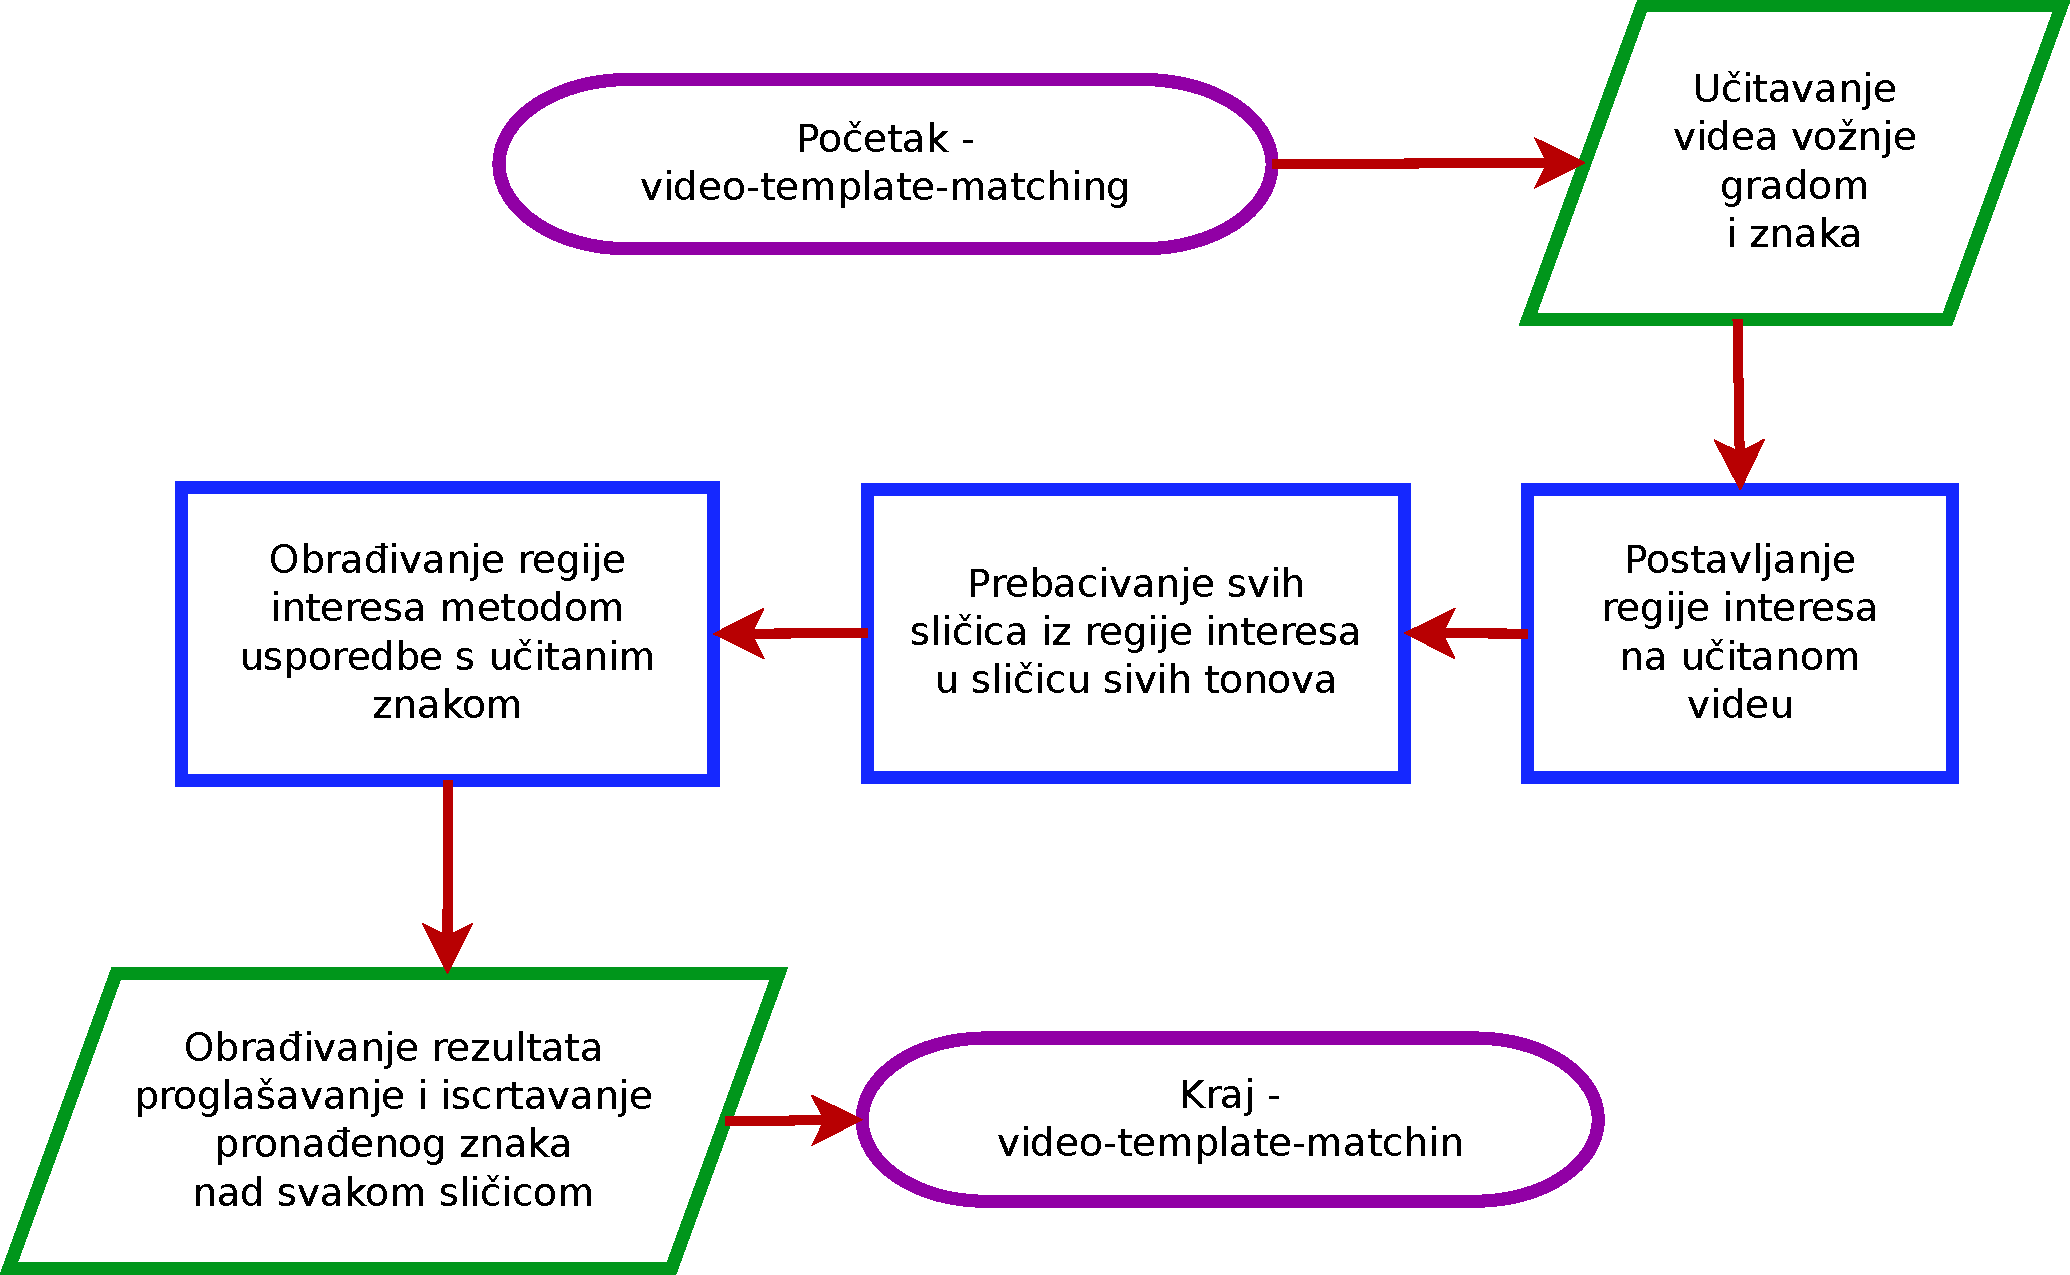
\includegraphics[scale=0.4]{figures/dijagramtoka.pdf}
\caption{Dijagram toka programa video-template-matching}
\label{fig:dijagramtoka.pdf}
\end{figure}



\newpage
\subsubsection{Učitavanje videa vožnje i učitavanje znaka} % (fold)
\label{ssub:Učitavanje videa vožnje i učitavanje znaka}


\begin{lstlisting}[label=lstUcit,caption={Izvorni kod za učitavanje
videa i znaka}]
#include "opencv2/imgproc/imgproc.hpp"

int main (int argc, char *argv[])
{
    // kreiranje objekta cap za ucitavanje videa
    VideoCapture cap("video/znakich2.mp4");
    if(!cap.isOpened())  // provjera uspjeha ucitavanja
        return -1;

    // kreiranje objekta Mat za spremanje znakova
    Mat znak1, znak2, znak3, znak4;

    // ucitavanje izrezanih znakova u razlicitim velicinama
    // trenutno se koristi samo znak2 
    znak1 = imread ("roi/01_roi.png");      
    znak2 = imread ("roi/02_roi.png");
    znak3 = imread ("roi/03_roi.png");
    znak4 = imread ("roi/04_roi.png");

}
\end{lstlisting}

Izlistanje koda~\ref{lstUcit} prikazuje primjer učitavanja videa i
učitavanje znaka upotrebom klase \texttt{VideoCapture} i funkcije
\texttt{imread} koji su uključeni dodavanjem biblioteke
\texttt{imgproc.hpp}. 
Slika \ref{fig:lstU} prikazuje učitan video i znak. 
Kreiranom objektu \texttt{cap} predana je putanja
do videa kojeg treba učitati. Ukoliko video nije uspješno učitan program
završava i vraća \texttt{-1}. Kreiranim objektima \texttt{znak1},
\texttt{znak2}, \texttt{znak3}, \texttt{znak4} pridružene su slike
učitane upotrebom funkcije \texttt{imread} kojoj je predana putanja do
slike koju treba učitati.

\begin{figure}[!htb]
\minipage{0.05\textwidth}
\endminipage\hfill
\minipage{0.5\textwidth}
    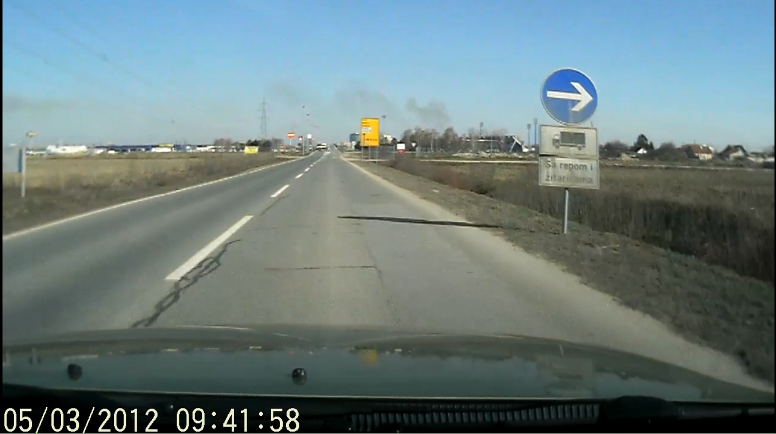
\includegraphics[width=\linewidth]{figures/scena.png}
\endminipage\hfill
\minipage{0.2\textwidth}
\endminipage\hfill
\minipage{0.2\textwidth}
    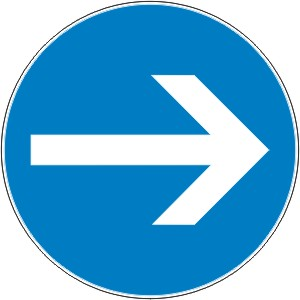
\includegraphics[width=\linewidth]{figures/znak.png}
\endminipage\hfill
\minipage{0.05\textwidth}
\endminipage\hfill
\caption{Prikaz učitanog videa (lijevo) i učitanog znaka (desno)}
\label{fig:lstU}
\end{figure}

% subsubsection Učitavanje videa vožnje i učitavanje znaka (end)

\newpage
\subsubsection{Postavljanje regije interesa} % (fold)
\label{ssub:Postavljanje regije interesa}


\begin{lstlisting}[label=lstRoi,caption={Izvorni kod za postvljanje
regije interesa}]
    // prebacivanje znak2 u sliku sivih nijansi
    cvtColor (znak2, znak2, CV_BGR2GRAY);
    
    // ucitavanje slicice iz videa u frame
    // postavljanje regije interesa u roi
    cap >> frame;
    rect = Rect (600, 150, 480, 120);
    roi = frame(rect);
    
\end{lstlisting}

Izlistanje koda~\ref{lstRoi} prikazuje upotrebu funkcije
\texttt{cvtColor} kojom se učitani znak prebacuje u sliku sivih tonova
kao što se vidi na slici \ref{fig:lstR}
Zatim se učitava sličica u objekt \texttt{frame} iz objekta
\texttt{cap}. Tada se kreira objekt \texttt{rect} pomoću funkcije
\texttt{Rect()} kojom definiramo pravokutnik koordinatama gornjeg
lijevog kuta te širinom i visinom. Takav pravokutnik upotrebljava se za
definiranje regije interesa nad učitanom sličicom odnosno objektom
\texttt{frame} te se regija interesa sprema u objekt \texttt{roi}.
Regija interesa se kasnije upotrebljava u algoritmu usporedbe s
predloškom.

\begin{figure}[!htb]
\minipage{0.05\textwidth}
\endminipage\hfill
\minipage{0.2\textwidth}
    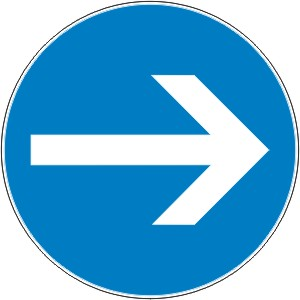
\includegraphics[width=\linewidth]{figures/znak.png}
\endminipage\hfill
\minipage{0.2\textwidth}
\endminipage\hfill
\minipage{0.2\textwidth}
    
\includegraphics[width=\linewidth]{figures/znakg.png}
\endminipage\hfill
\minipage{0.05\textwidth}
\endminipage\hfill
\caption{Prikaz prebacivanja učitanog znak u sliku sivih tonova}
\label{fig:lstR}
\end{figure}


% subsubsection Postavljanje regije interesa (end)

\newpage
\subsubsection{Pozivanje algoritma usporedbe s predloškom} % (fold)
\label{ssub:Pozivanje algoritma usporedbe s predloškom}

\begin{lstlisting}[label=lstTemp,caption={Izvorni kod pozivanja
algoritma usporedbe s predloškom}]
    // postavljanje velicine results ovisno o velicini roi i znak2
    int resultRows, resultCols;
    resultRows = roi.rows - znak2.rows + 1;
    resultCols = roi.cols - znak2.cols + 1;
    results.create (resultRows, resultCols, CV_32FC1);

    // pretvaranje roi u greyscale
    cvtColor(roi, groi, CV_BGR2GRAY);      
    // trazenje znaka u greyscale groi i spremanje u results
    // matematicke funkcije za racunanje rezultatne matrice
    // 0: SQDIFF, 1: SQDIFF NORMED, 2: TM CCORR,  
    // 3: TM CCORR NORMED, 4: TM COEFF, 5: TM COEFF NORMED
    matchTemplate (groi, znak2, results, 5);
    // normaliziranje rezultata
    normalize (results, results, 0, 1, NORM_MINMAX, -1);
    // traznje lokacije najveceg rezultata
    double minVal; double maxVal;
    minMaxLoc (results, &minVal, &maxVal, &minLoc, &maxLoc, Mat() );
    // spremanje rezultata u vektor tocaka
    vPoint.push_back (maxLoc);

\end{lstlisting}

Prije pozivanja algoritma usporedbe s predloškom implementiranog u
funkciji \texttt{matchTemplate()} potrebno je kreirati matricu/sliku u
koju će funkcija spremati rezultate. Matrica \texttt{results} se kreira
ovisno o veličini matrica \texttt{roi} i \texttt{znak2} kao što
prikazuje izlistanje koda~\ref{lstTemp} Kako su svi parametri koje
funkcija \texttt{matchTemplate()} prima kreirani, slijedi njeno pozivanje. Predani parametri se vide i na slici \ref{fig:mt}
Funkcija je pozvana s zadnjim parametrom 5 koji označava da se korsiti 
matematička funkcija \texttt{TM\_CCORR\_NORMED} za računanje rezultantne
matrice. Korištena funkcija slične piksele (pozitivne rezultate) prikazuje
svijetlom nijansom sive boje.
Rezultat rada algoritma je spremljen u \texttt{results} te se takvi
rezultati normaliziraju korištenjem funkcije \texttt{normalize()}. Zatim
slijedi lociranje najvećih i najmanjih vrijednosti piksela u rezultantnoj
matrici upotrebom funkcije \texttt{minMaxLoc()}. Korištena metoda
usporedbe sprema najbolje rezultate kao maksimalne vrijednosti i zato se
\texttt{maxLoc} sprema u vektor točaka za daljnju obradu.

\begin{figure}[!htb]
\minipage{0.35\textwidth}
    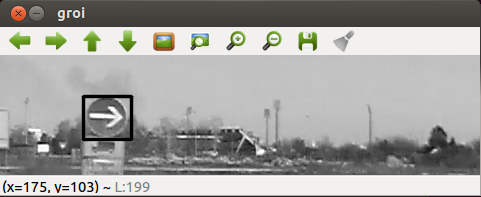
\includegraphics[width=\linewidth]{figures/mt-groi.png}
\endminipage\hfill
\minipage{0.75\textwidth}
\endminipage\hfill
\minipage{0.05\textwidth}
    
\includegraphics[width=\linewidth]{figures/znakg.png}
\endminipage\hfill
\minipage{0.75\textwidth}
\endminipage\hfill
\minipage{0.35\textwidth}
    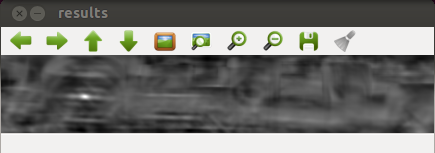
\includegraphics[width=\linewidth]{figures/mt-results.png}
\endminipage\hfill

\caption{Prikaz predanih parametra \texttt{matchTemplate} funkciji:
regija interesa (lijevo), predložak (sredina)
i dobiveni rezultata (desno)}
\label{fig:mt}
\end{figure}

\newpage
\subsubsection{Eliminacija lažno pozitivnih rezultata} % (fold)
\label{ssub:Eliminacija lažno pozitivnih rezultata}

Zbog velike količine lažno pozitivnih rezultata osmišljen je kod za
eliminaciju istih računanjem geometrijske udaljenosti između dvije
točke. Kod za računanje geometrijske udaljenosti je prikazan u ispisu
koda~\ref{lstDist}, a primjer lažno detektiranog znaka se vidi na slici
\ref{fig:ld1} Pretpostavka je da se znak pojavljuje postepeno što
znači da bi rezultati trebali biti u blizini prošlog rezultata odnosno ne
bi trebali iznenadno pojavljivati na velikim udaljenostima između
uzastopnih sličica. 

\begin{lstlisting}[label=lstDist,caption={Izvorni kod računanja
geometrijske udaljenosti između dvije točke}]
int calcPointDist (Point maxLoc, Point prevMaxLoc)
{
    int dist = 0;
    dist = sqrt ((maxLoc.x - prevMaxLoc.x) * (maxLoc.x - prevMaxLoc.x) +
                 (maxLoc.y - prevMaxLoc.y) * (maxLoc.y - prevMaxLoc.y));    
    cout << dist << endl;
    return dist;
}
\end{lstlisting}

Kao što se vidi iz ispisa koda~\ref{lstFP} program ima beskonačnu petlju
u kojoj učitava sličicu po sličicu te nad svakom od njih ponovo poziva
algoritam usporedbe s predloškom, pronalazi najveće vrijednosti te 
iste sprema u vektor točka \texttt{vPoint}. 

\begin{lstlisting}[label=lstFP,caption={Izvorni kod obrade svih učitanih
        sličica }]
for (;;){
    // ucitaj frame, postavi roi, prebaci u greyscale
    cap >> frame;              
    roi = frame(rect);
    cvtColor(roi, groi, CV_BGR2GRAY);
    
    matchTemplate (groi, znak2, results, 5);
    normalize (results, results, 0, 1, NORM_MINMAX, -1);
    minMaxLoc (results, &minVal, &maxVal, &minLoc, &maxLoc, Mat() );
    vPoint.push_back (maxLoc);
    int size = vPoint.size();
\end{lstlisting}
    
Za svaki rezultat veći od postavljene vrijednosti (0.75) izvršava se
logika koja određuje hoće li se prepoznati znak odnosno iscrtati
pravokutnik oko njega. Za prvih 10 \texttt{maxVal} vrijednosti većih od
0.75 znak se prepoznaje ako je udaljenost između početne i trenutne
vrijednosti manja od 10. Za ostale rezultate uspoređuje se trenutni i
sedmi prije. Ukoliko je udaljenost između njih veća od 15 znak se
prepoznaje i iscrtava. Kod vidljiv u ispisu~\ref{lstFP2} još prikazuje
ponovno stavljanje iste točke u vektor zbog dužeg prikaza/praćenja
znaka. 

\newpage
\begin{lstlisting}[label=lstFP2,caption={Izvorni kod eliminacije
lažno pozitivnih rezultata}]
    // Za svaki rezultat veci od 0.75 
    if (maxVal > 0.75) {
        // racunaj udaljenost izmedu dva rezultata
        // Ako je vektor tocaka manji od 10 clanova
        if (size < 10) {
            // racunaj udaljenost izmedu trenutne i prve tocke
            dist = calcPointDist (maxLoc, vPoint.at(0));
            // ako je udaljenost manja od 10 isrctaj znak
            if (dist < 10) {
                rectangle (groi, maxLoc, Point(maxLoc.x + znak2.cols, 
                maxLoc.y + znak2.rows), Scalar::all(0), 2, 18, 0 );
            }
        }
        // Ako je vektor tocaka veci od 10 clanova
        else {
            // racunaj udaljenost izmedu trenutnog i sedomog prije 
            dist = calcPointDist (maxLoc, vPoint.at(size-7));  
            // iscrtaj pravokutnik ako je udaljenost manja od 15 
            if (dist < 15) {
                rectangle (groi, maxLoc, Point(maxLoc.x + znak2.cols, 
                maxLoc.y + znak2.rows), Scalar::all(0), 2, 18, 0 );
                // ponovi istu tocku u vektor da se duze prati znak
                vPoint.push_back (maxLoc);  
            }
            else {
            // ponovi istu tocku u vektor da se duze prati znak
            vPoint.push_back (maxLoc);
            }
        }
    }
}
\end{lstlisting}

\begin{figure}[!htb]
\minipage{0.15\textwidth}
\endminipage\hfill
\minipage{0.5\textwidth}
    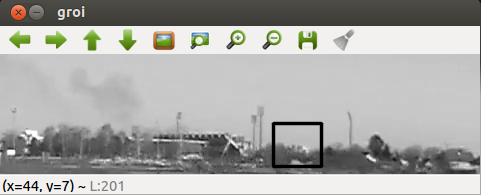
\includegraphics[width=\linewidth]{figures/ld1.png}
\endminipage\hfill
\minipage{0.05\textwidth}
    
\includegraphics[width=\linewidth]{figures/znakg.png}
\endminipage\hfill
\minipage{0.15\textwidth}
\endminipage\hfill
\caption{Prikaz krivo detektiranog znaka (lažno pozitivan rezultat)
(lijevo) i znaka koji se traži (desno)}
\label{fig:ld1}
\end{figure}


% subsubsection Eliminacija lažno pozitivnih rezultata (end)

% subsubsection Pozivanje algoritma usporedbe s predloškom (end)

% subsection Prepoznavanje (end)

% section Prepoznavanje prometnog (end)
